\subsubsection{Attori}
In questa sezione, per la definizione degli attori abbiamo deciso di riutilizzare le persona definite in § Persona.
Sebbene le avessimo già dettagliate abbondantemente nella fase dello Studio di Fattibilità, abbiamo ritenuto significativo caratterizzarle anche mediante il \textit{Diagramma C\&A} nei termini delle sei caratteristiche maggiormente impattanti le scelte progettuali: competenza tecnica, di dominio, di linguaggio, abilità fisiche, motivazione e concentrazione.

\noindent
\paragraph{Attori diretti e indiretti}\mbox{}\\
Gli attori cui siamo pervenuti pertanto sono:
\begin{itemize}
    \item Diretti:
    \begin{itemize}
        \item Fruizione:
        \begin{itemize}
            \item Giornalista di una testata nazionale;
            \item Giornalista d'agenzia;
            \item Giornalista di una testata locale;
            \item Cittadino esperto;
            \item Blogger;
        \end{itemize}
    \end{itemize}
    \item Indiretti:
    \begin{itemize}
        \item Amministrazione database e dashboard:
        \begin{itemize}
            \item Amministratore di database;
        \end{itemize}
        \item Fruizione da dispositivo mobile:
        \begin{itemize}
            \item Cittadino che visita la dashboard da un dispositivo mobile.
        \end{itemize}
    \end{itemize}
\end{itemize}

\paragraph{Diagrammi C\&A}\mbox{}\\
Abbiamo caratterizzato ogni attore individuato in base alle competenze e abilità che presenta e che impattano in maniera più significativa le scelte progettuali, per poi mappare ciascuno sul Diagramma C\&A, così da averne una visione d'insieme.
Ci siamo concentrati sugli attori diretti, articolando l'analisi tra le persona protagoniste (giornalisti) e le persona secondarie (blogger e cittadino esperto).\\
Il risultato ottenuto si può vedere nei successivi diagrammi:
\begin{figure}[H]
    \centering
    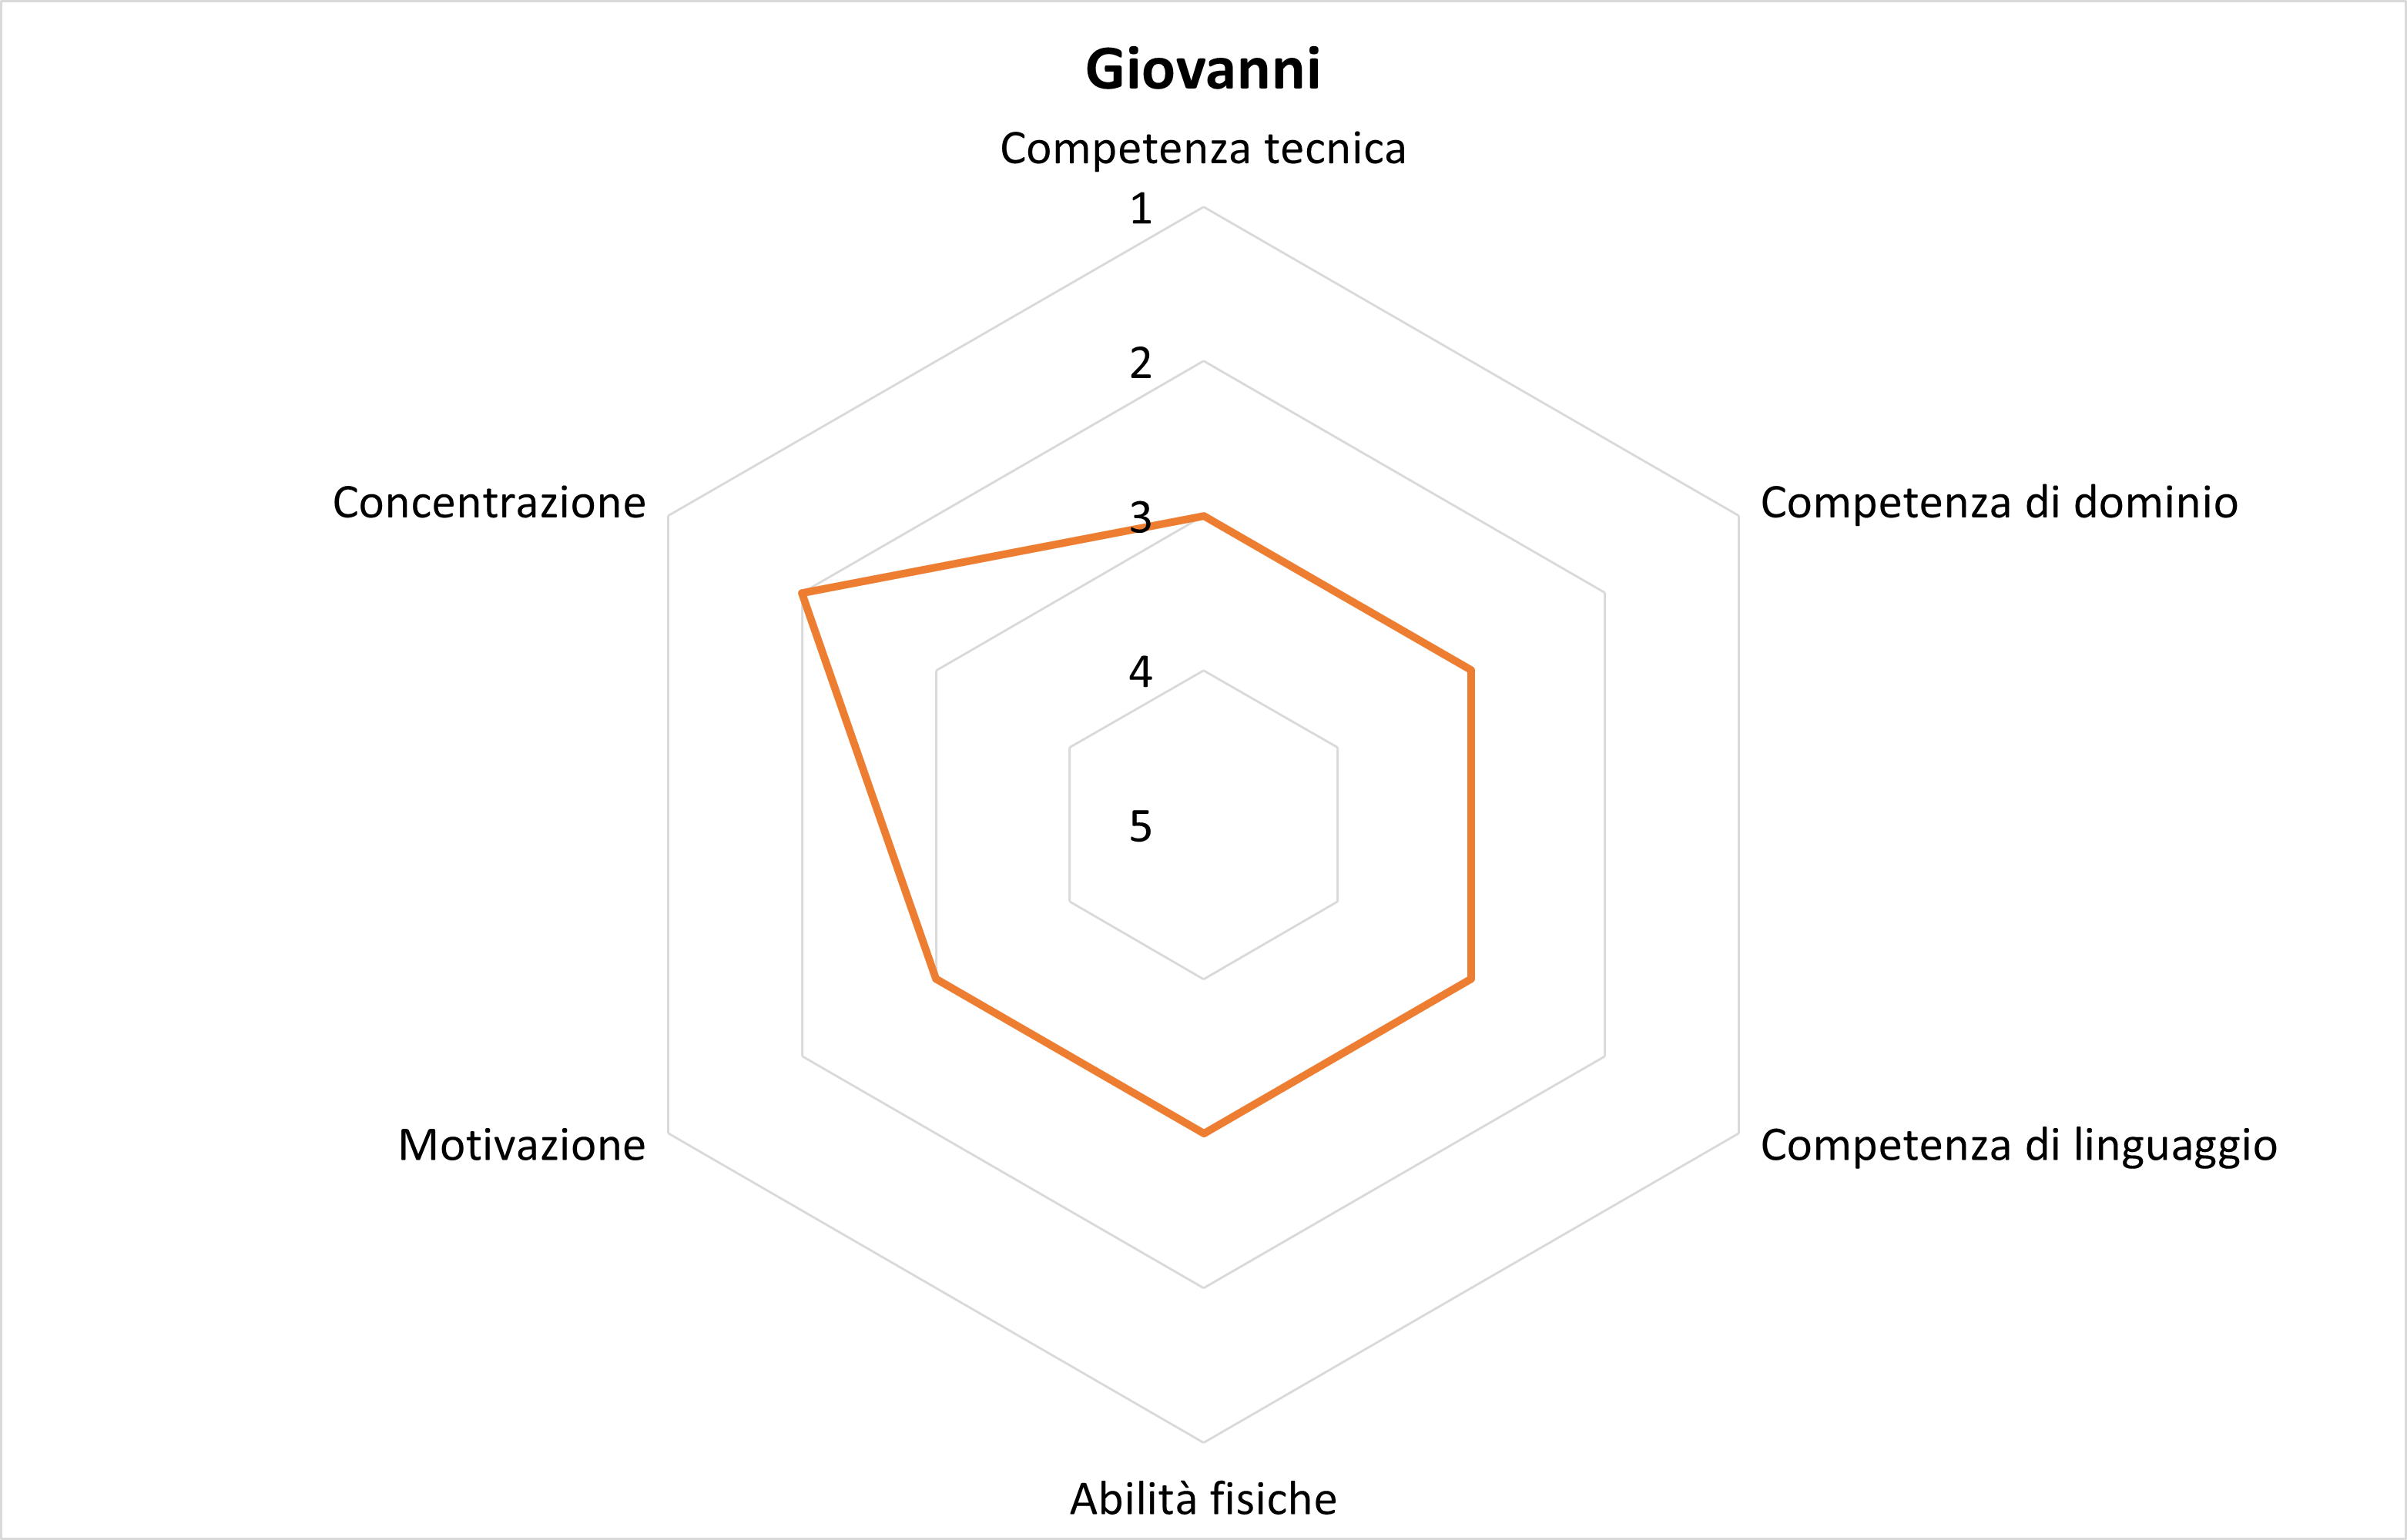
\includegraphics[width=0.5\columnwidth]{assets/images/proposta-design/caos/giovanni}
    \caption{Diagramma C\&A per Giovanni, il giornalista di una testata nazionale.}
\end{figure}

\begin{figure}[H]
    \centering
    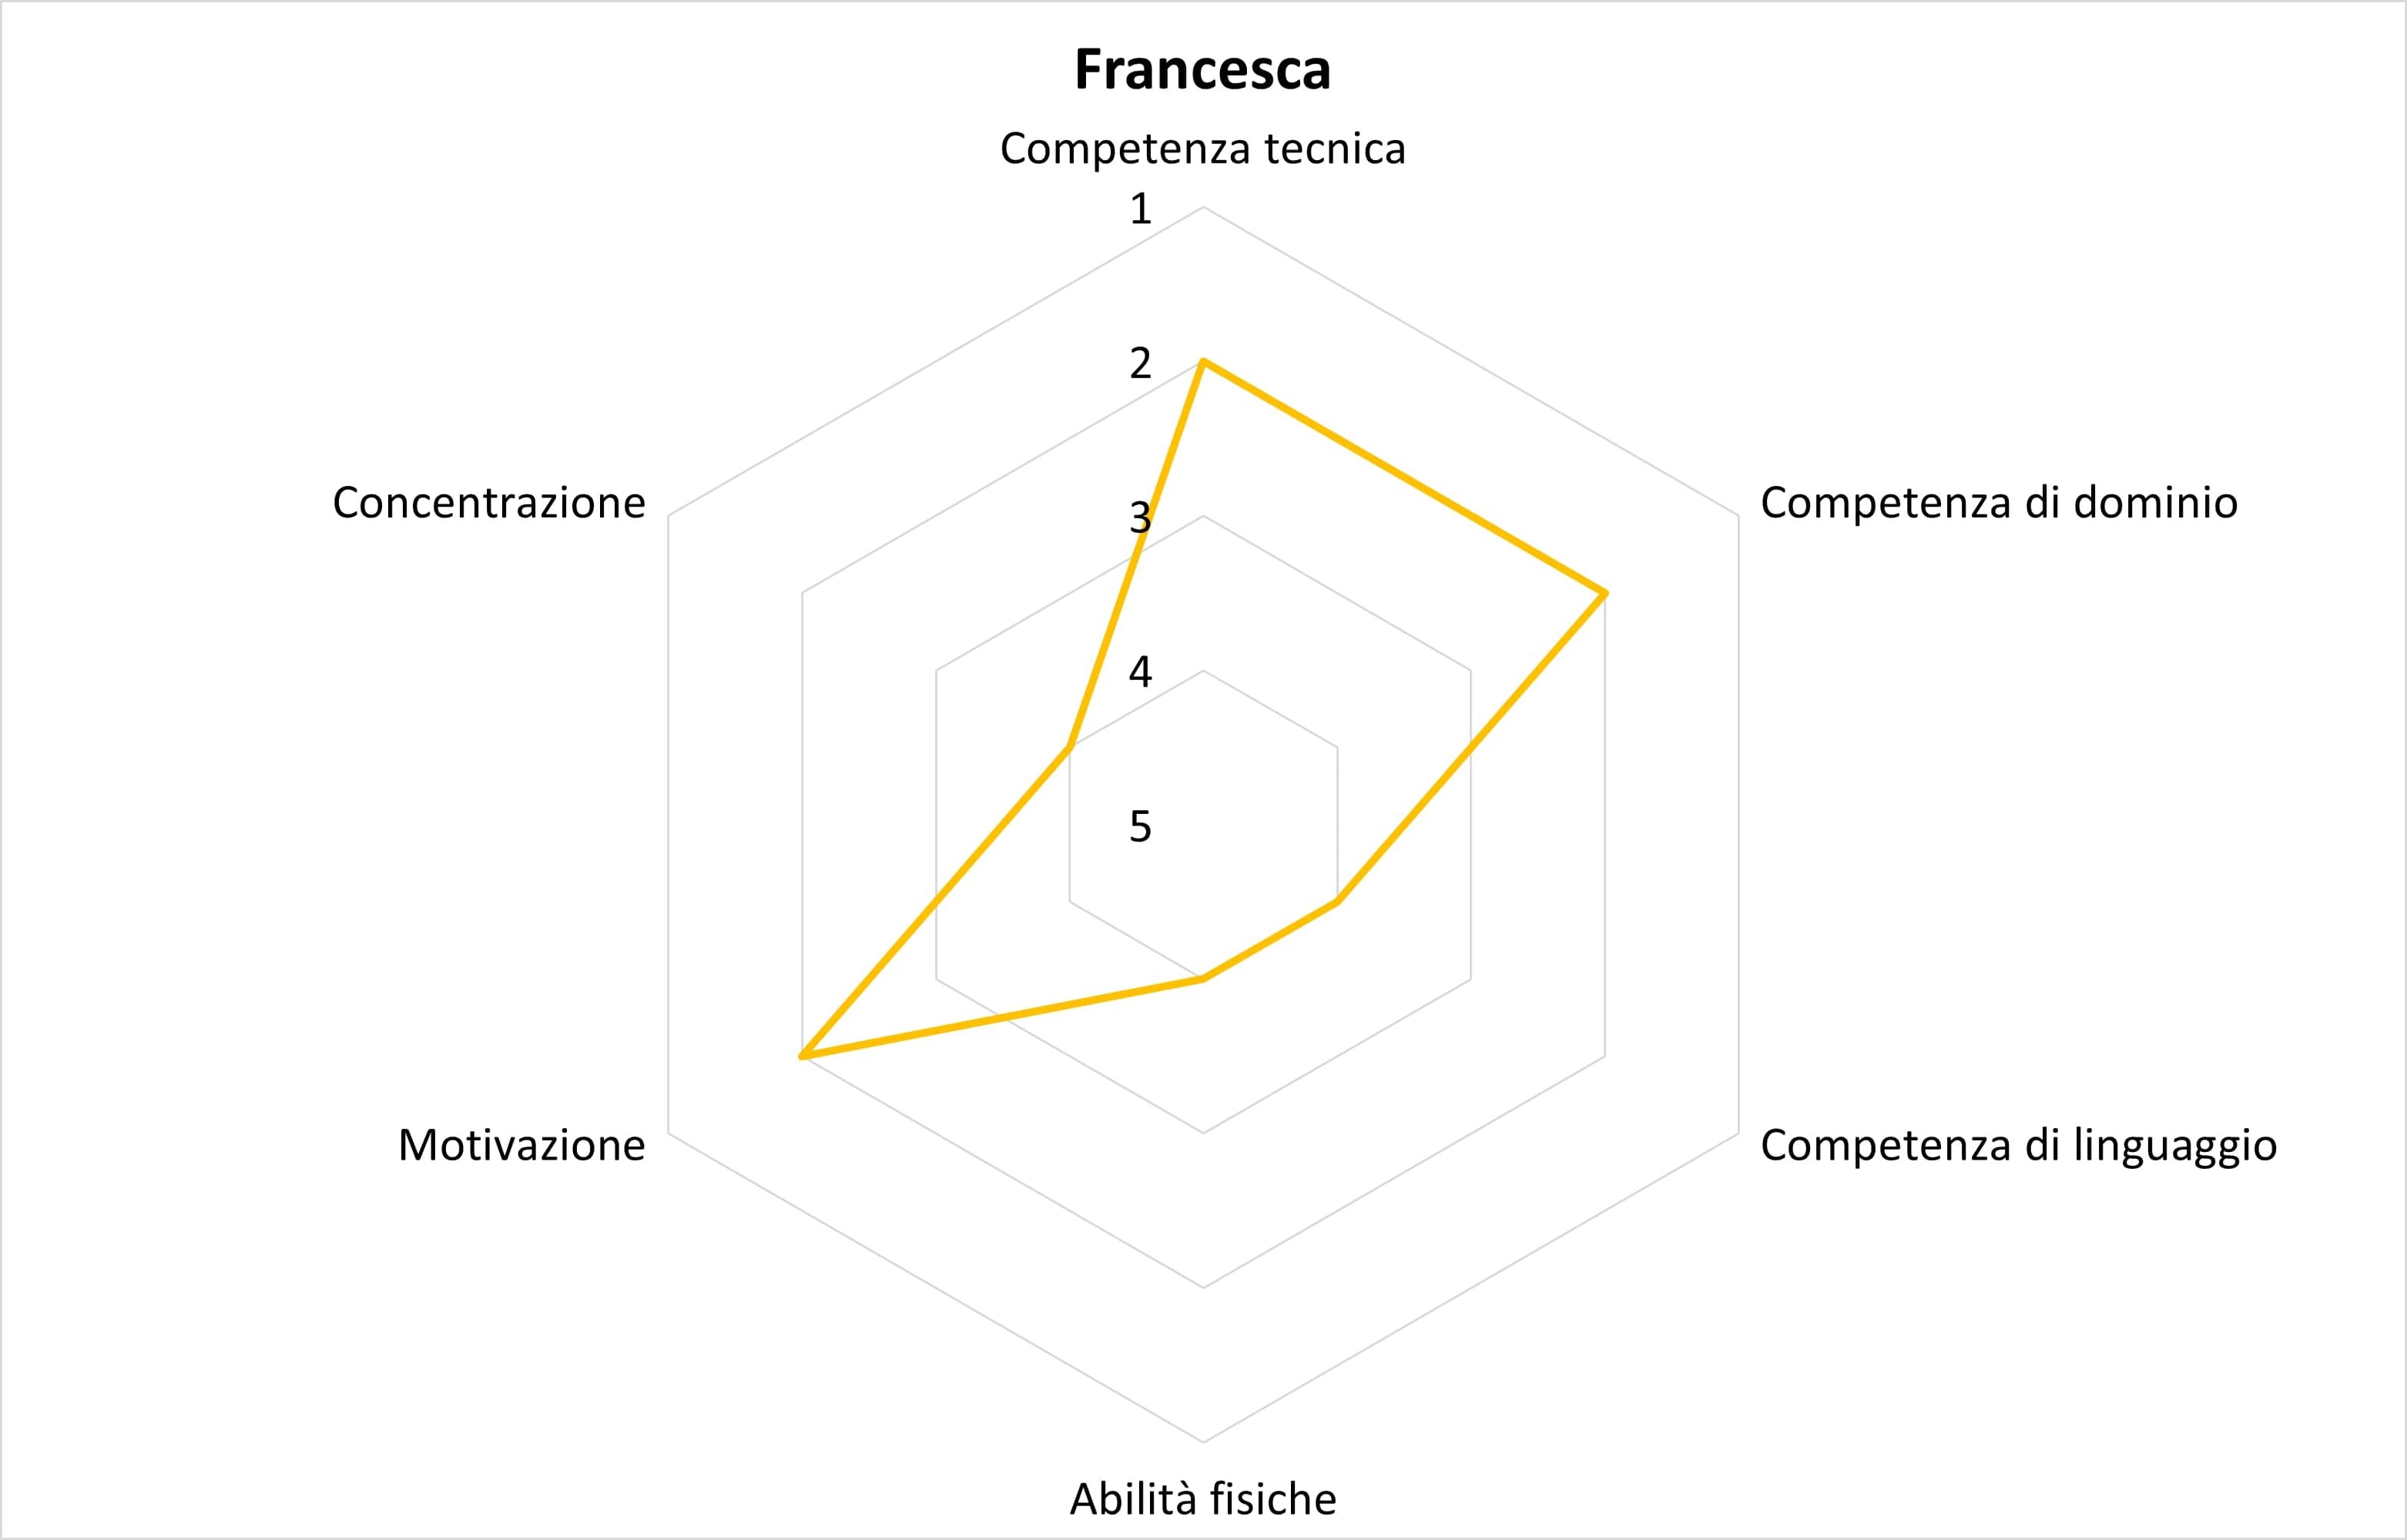
\includegraphics[width=0.5\columnwidth]{assets/images/proposta-design/caos/francesca}
    \caption{Diagramma C\&A per Francesca, la giornalista di una testata locale.}
\end{figure}

\begin{figure}[H]
    \centering
    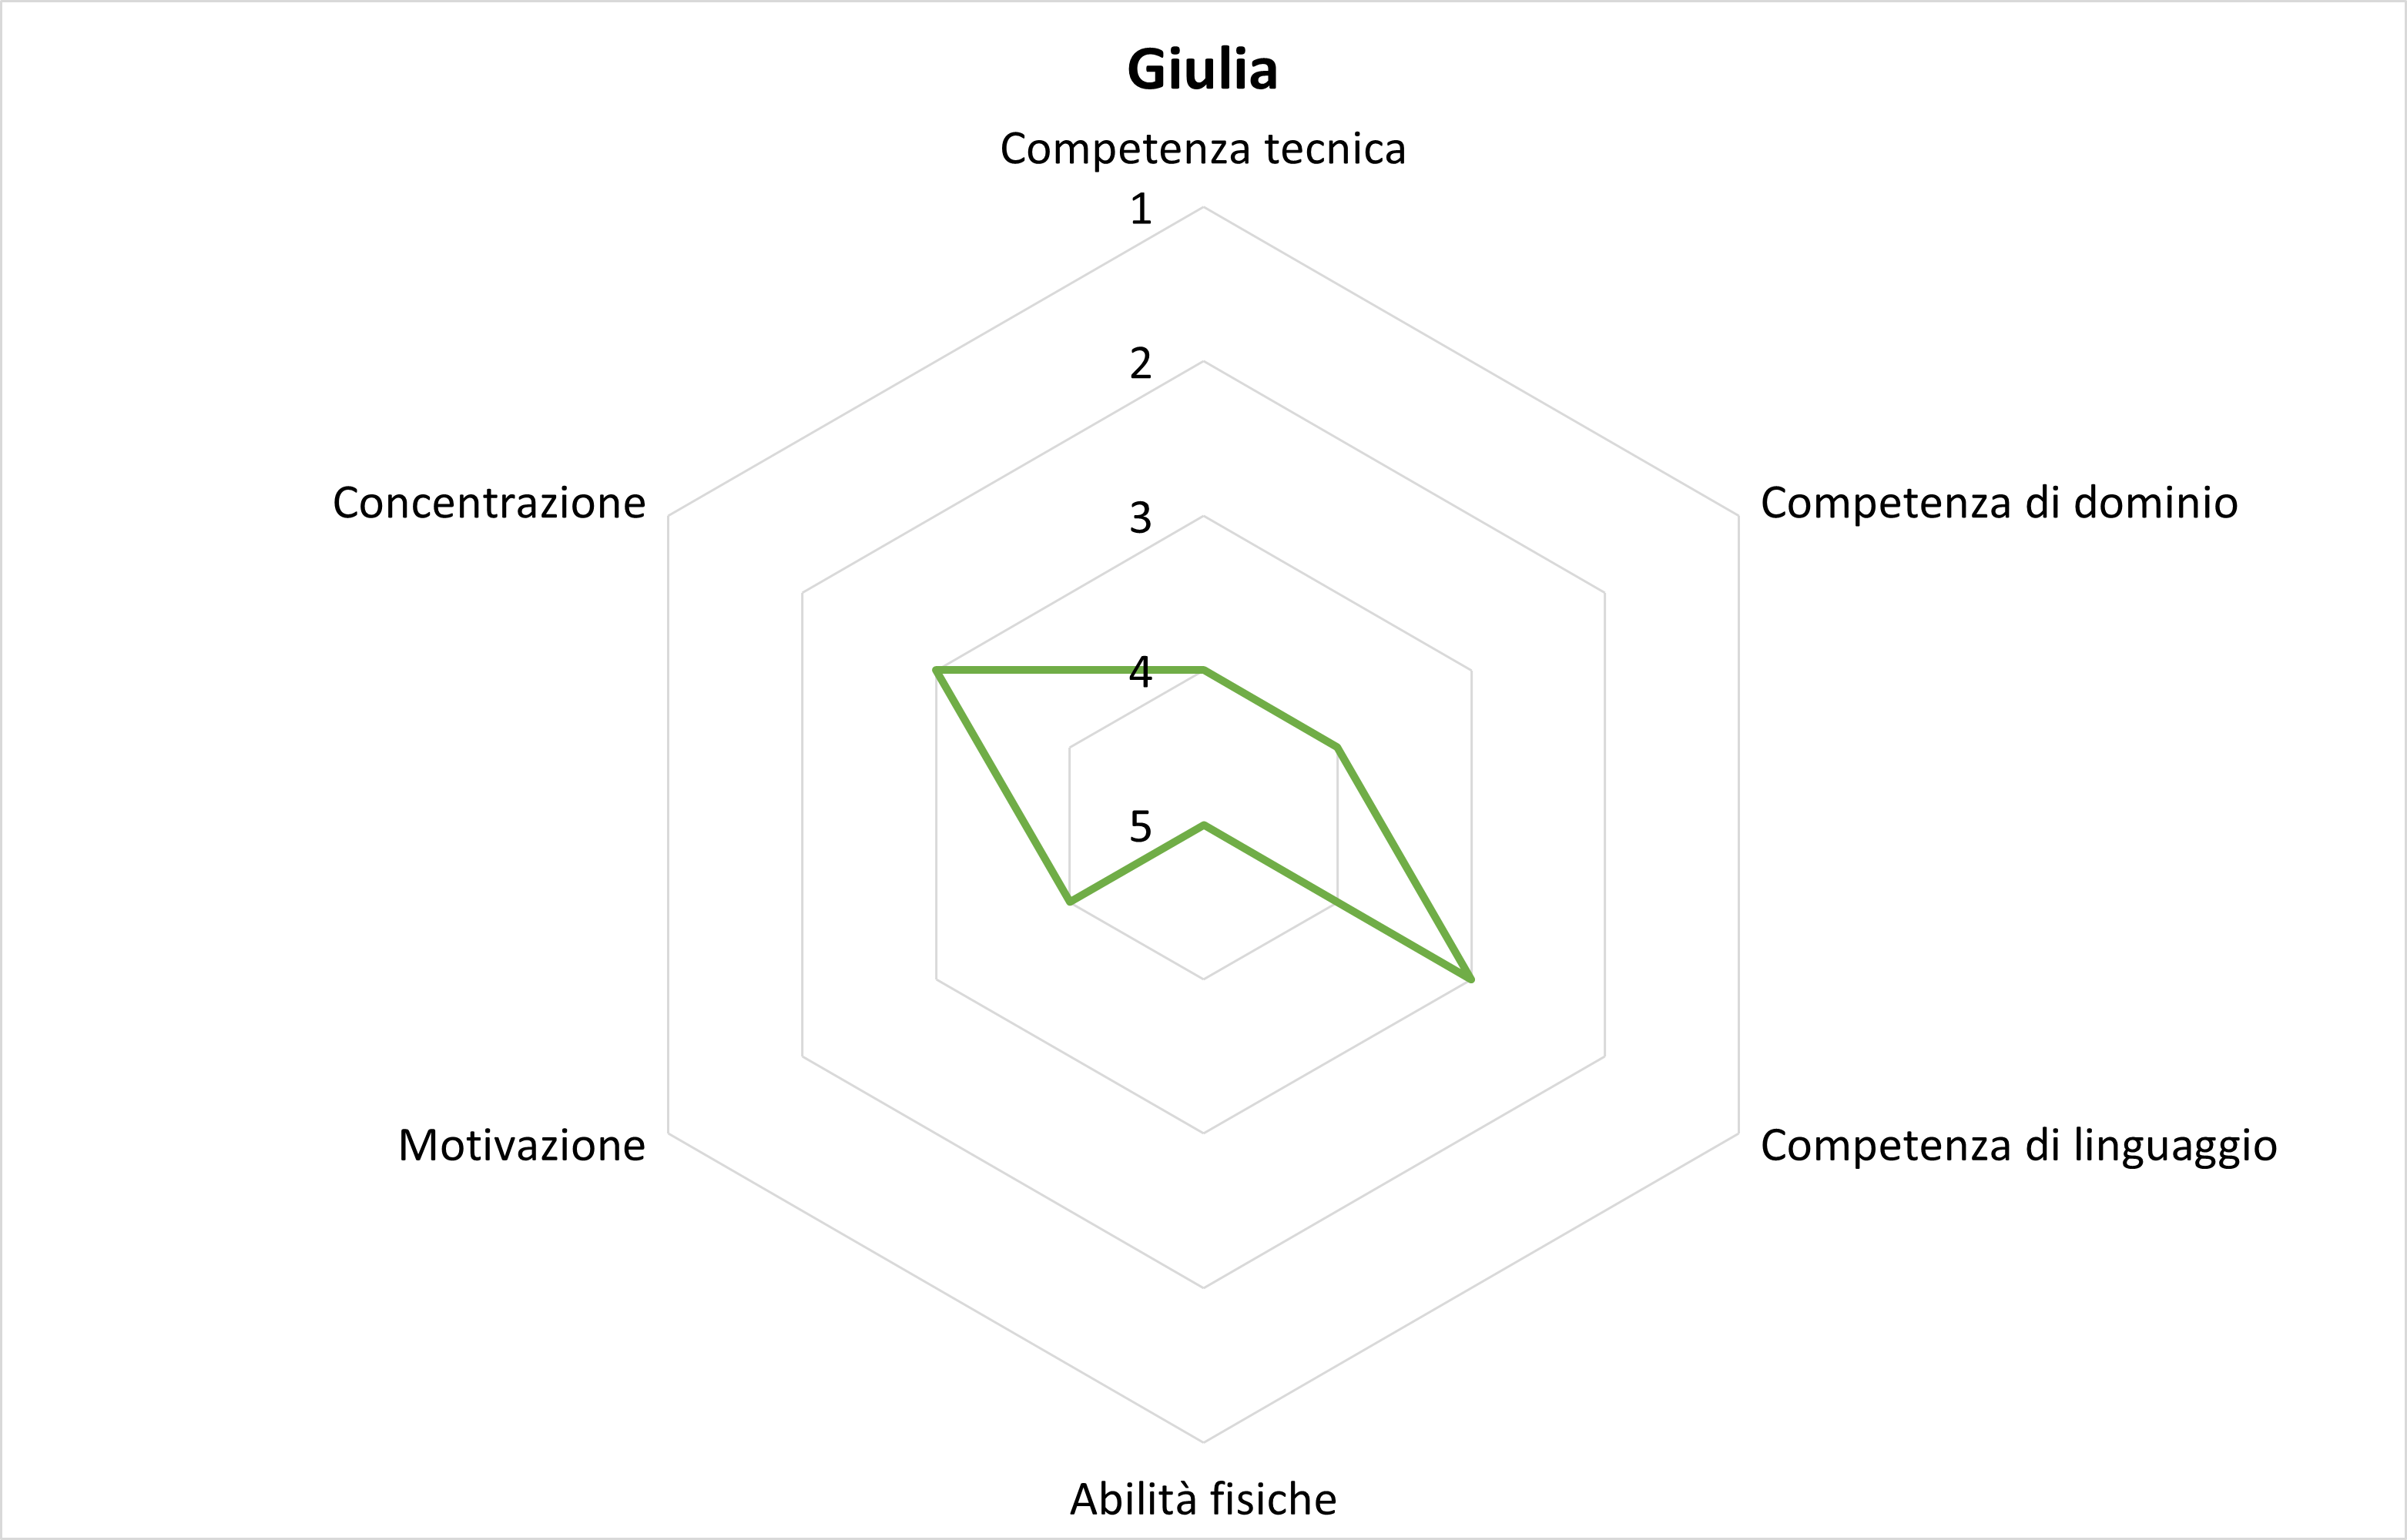
\includegraphics[width=0.5\columnwidth]{assets/images/proposta-design/caos/giulia}
    \caption{Diagramma C\&A per Giulia, la giornalista di una agenzia di stampa.}
\end{figure}

\begin{figure}[H]
    \centering
    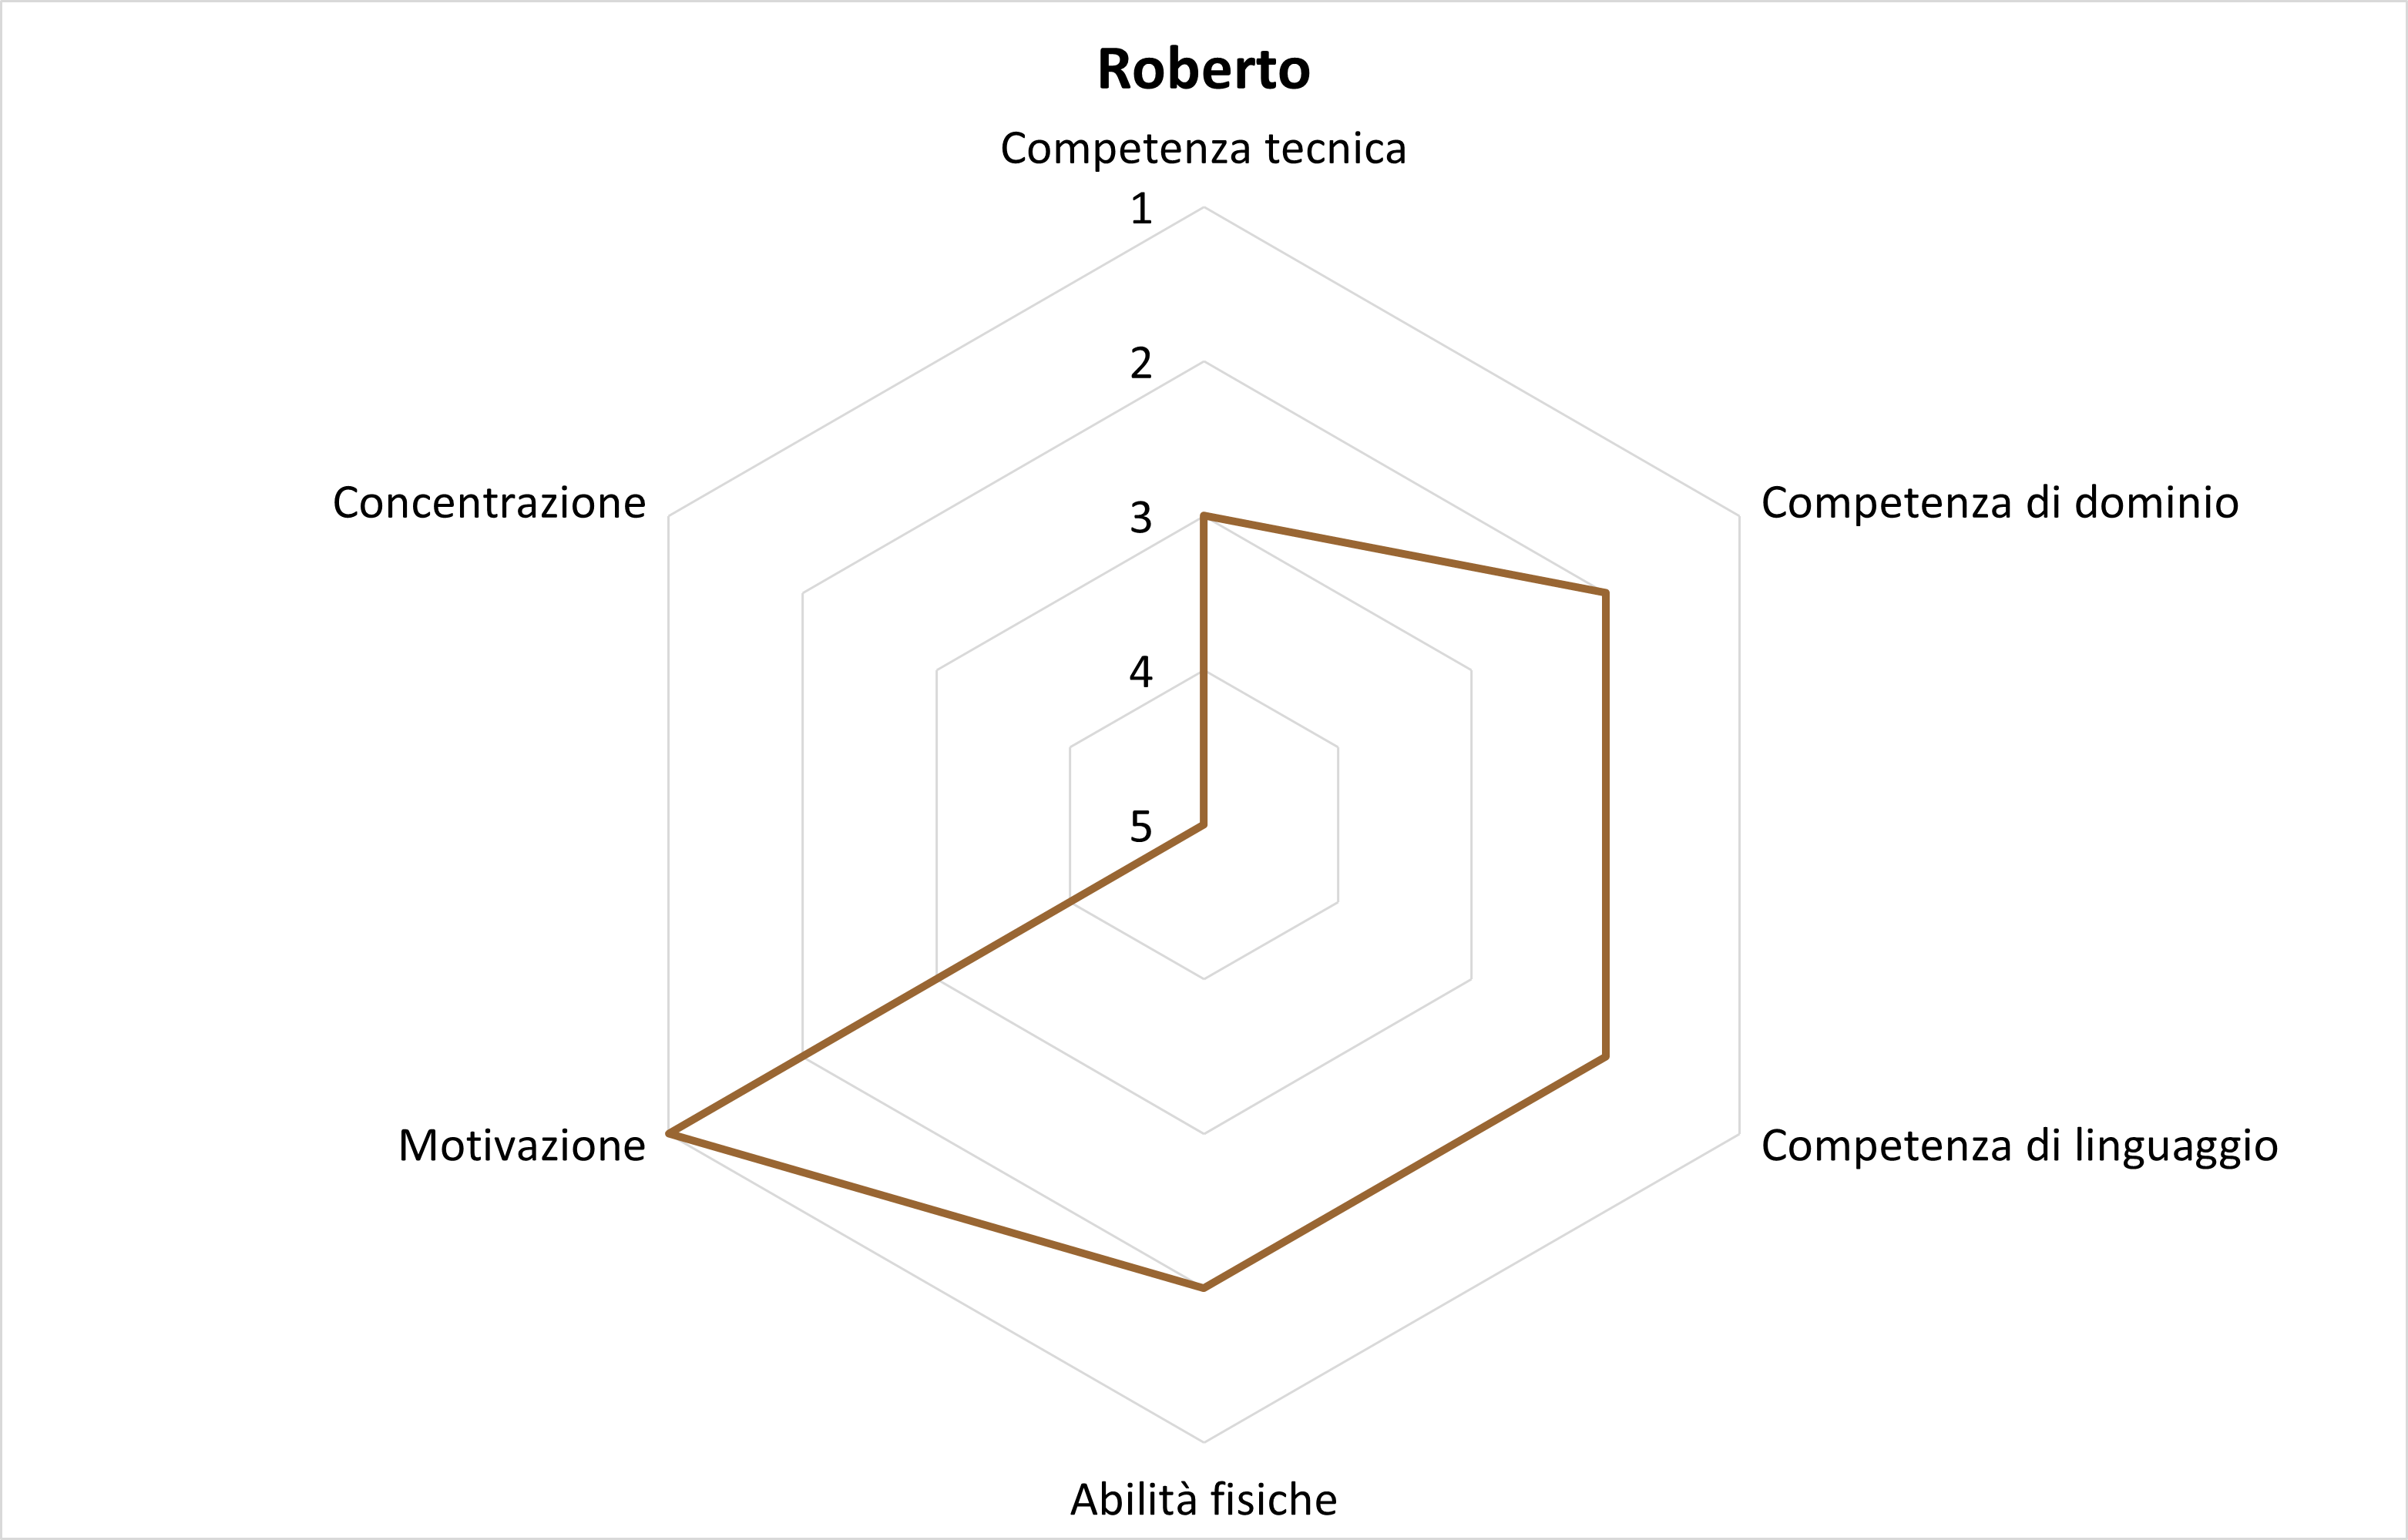
\includegraphics[width=0.5\columnwidth]{assets/images/proposta-design/caos/roberto}
    \caption{Diagramma C\&A per Roberto, il blogger.}
\end{figure}

\begin{figure}[H]
    \centering
    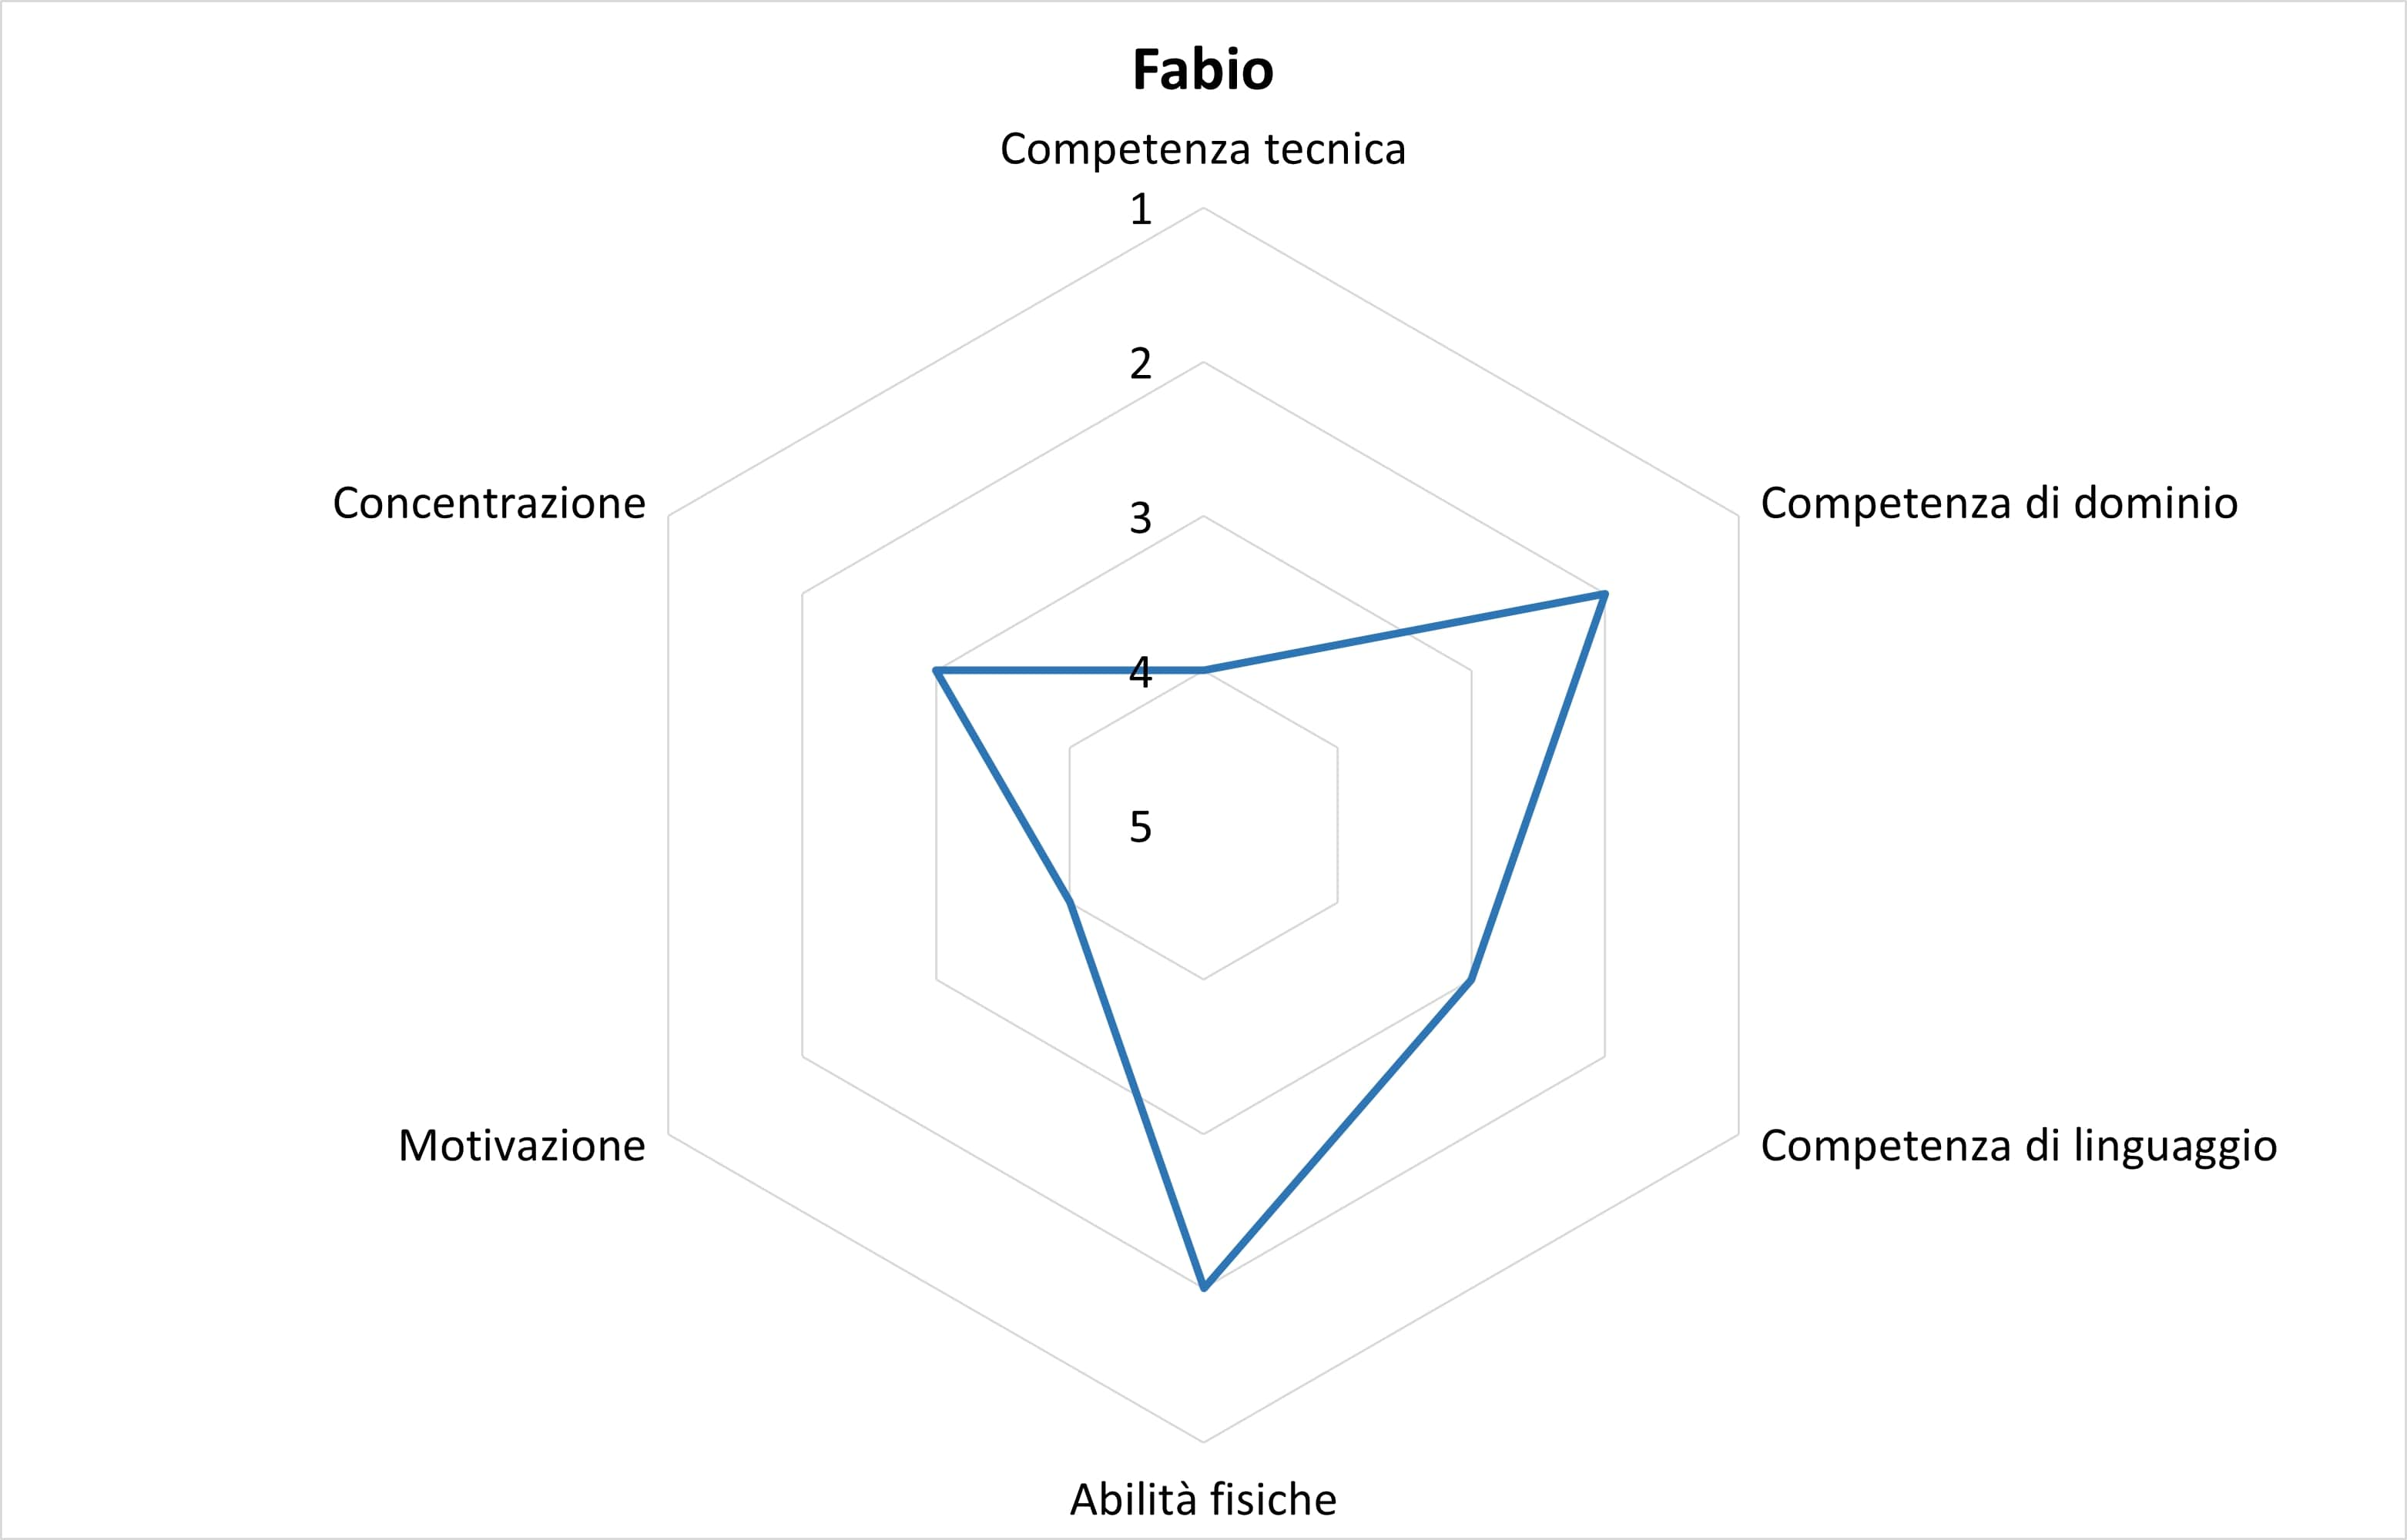
\includegraphics[width=0.5\columnwidth]{assets/images/proposta-design/caos/fabio}
    \caption{Diagramma C\&A per Fabio, il cittadino esperto.}
\end{figure}

\noindent
Per quanto riguarda i giornalisti, è emerso che le loro competenze sono in generale carenti su quelle tecniche e di dominio, rendendoli inclini alla possibilità di compiere errori (\textit{mistake}\footnote{Con il termine \textit{mistake} si intende un'errata comprensione del problema, con la conseguenza di commettere azioni sbagliate.}), per cui nella nostra riprogettazione della dashboard abbiamo previsto numerose spiegazioni on-demand sulle componenti trattanti concetti più complicati.
Inoltre, questi attori risultano essere affetti da scarsa concentrazione a causa dell'ambiente in cui operano, nonché bassa motivazione per via della volontarietà di adozione della dashboard tra varie alternative.
Pertanto, per invogliare gli utenti a consultare la dashboard oggetto della nostra riprogettazione, abbiamo posto l'enfasi sull'autorevolezza dell'istituzione che la gestisce, mentre per facilitare l'interazione anche in contesti con tante distrazioni, abbiamo previsto un'interfaccia chiara, consistente e che non richiede particolari carichi cognitivi, grazie alle sue numerose componenti grafiche.
\begin{figure}[H]
    \centering
    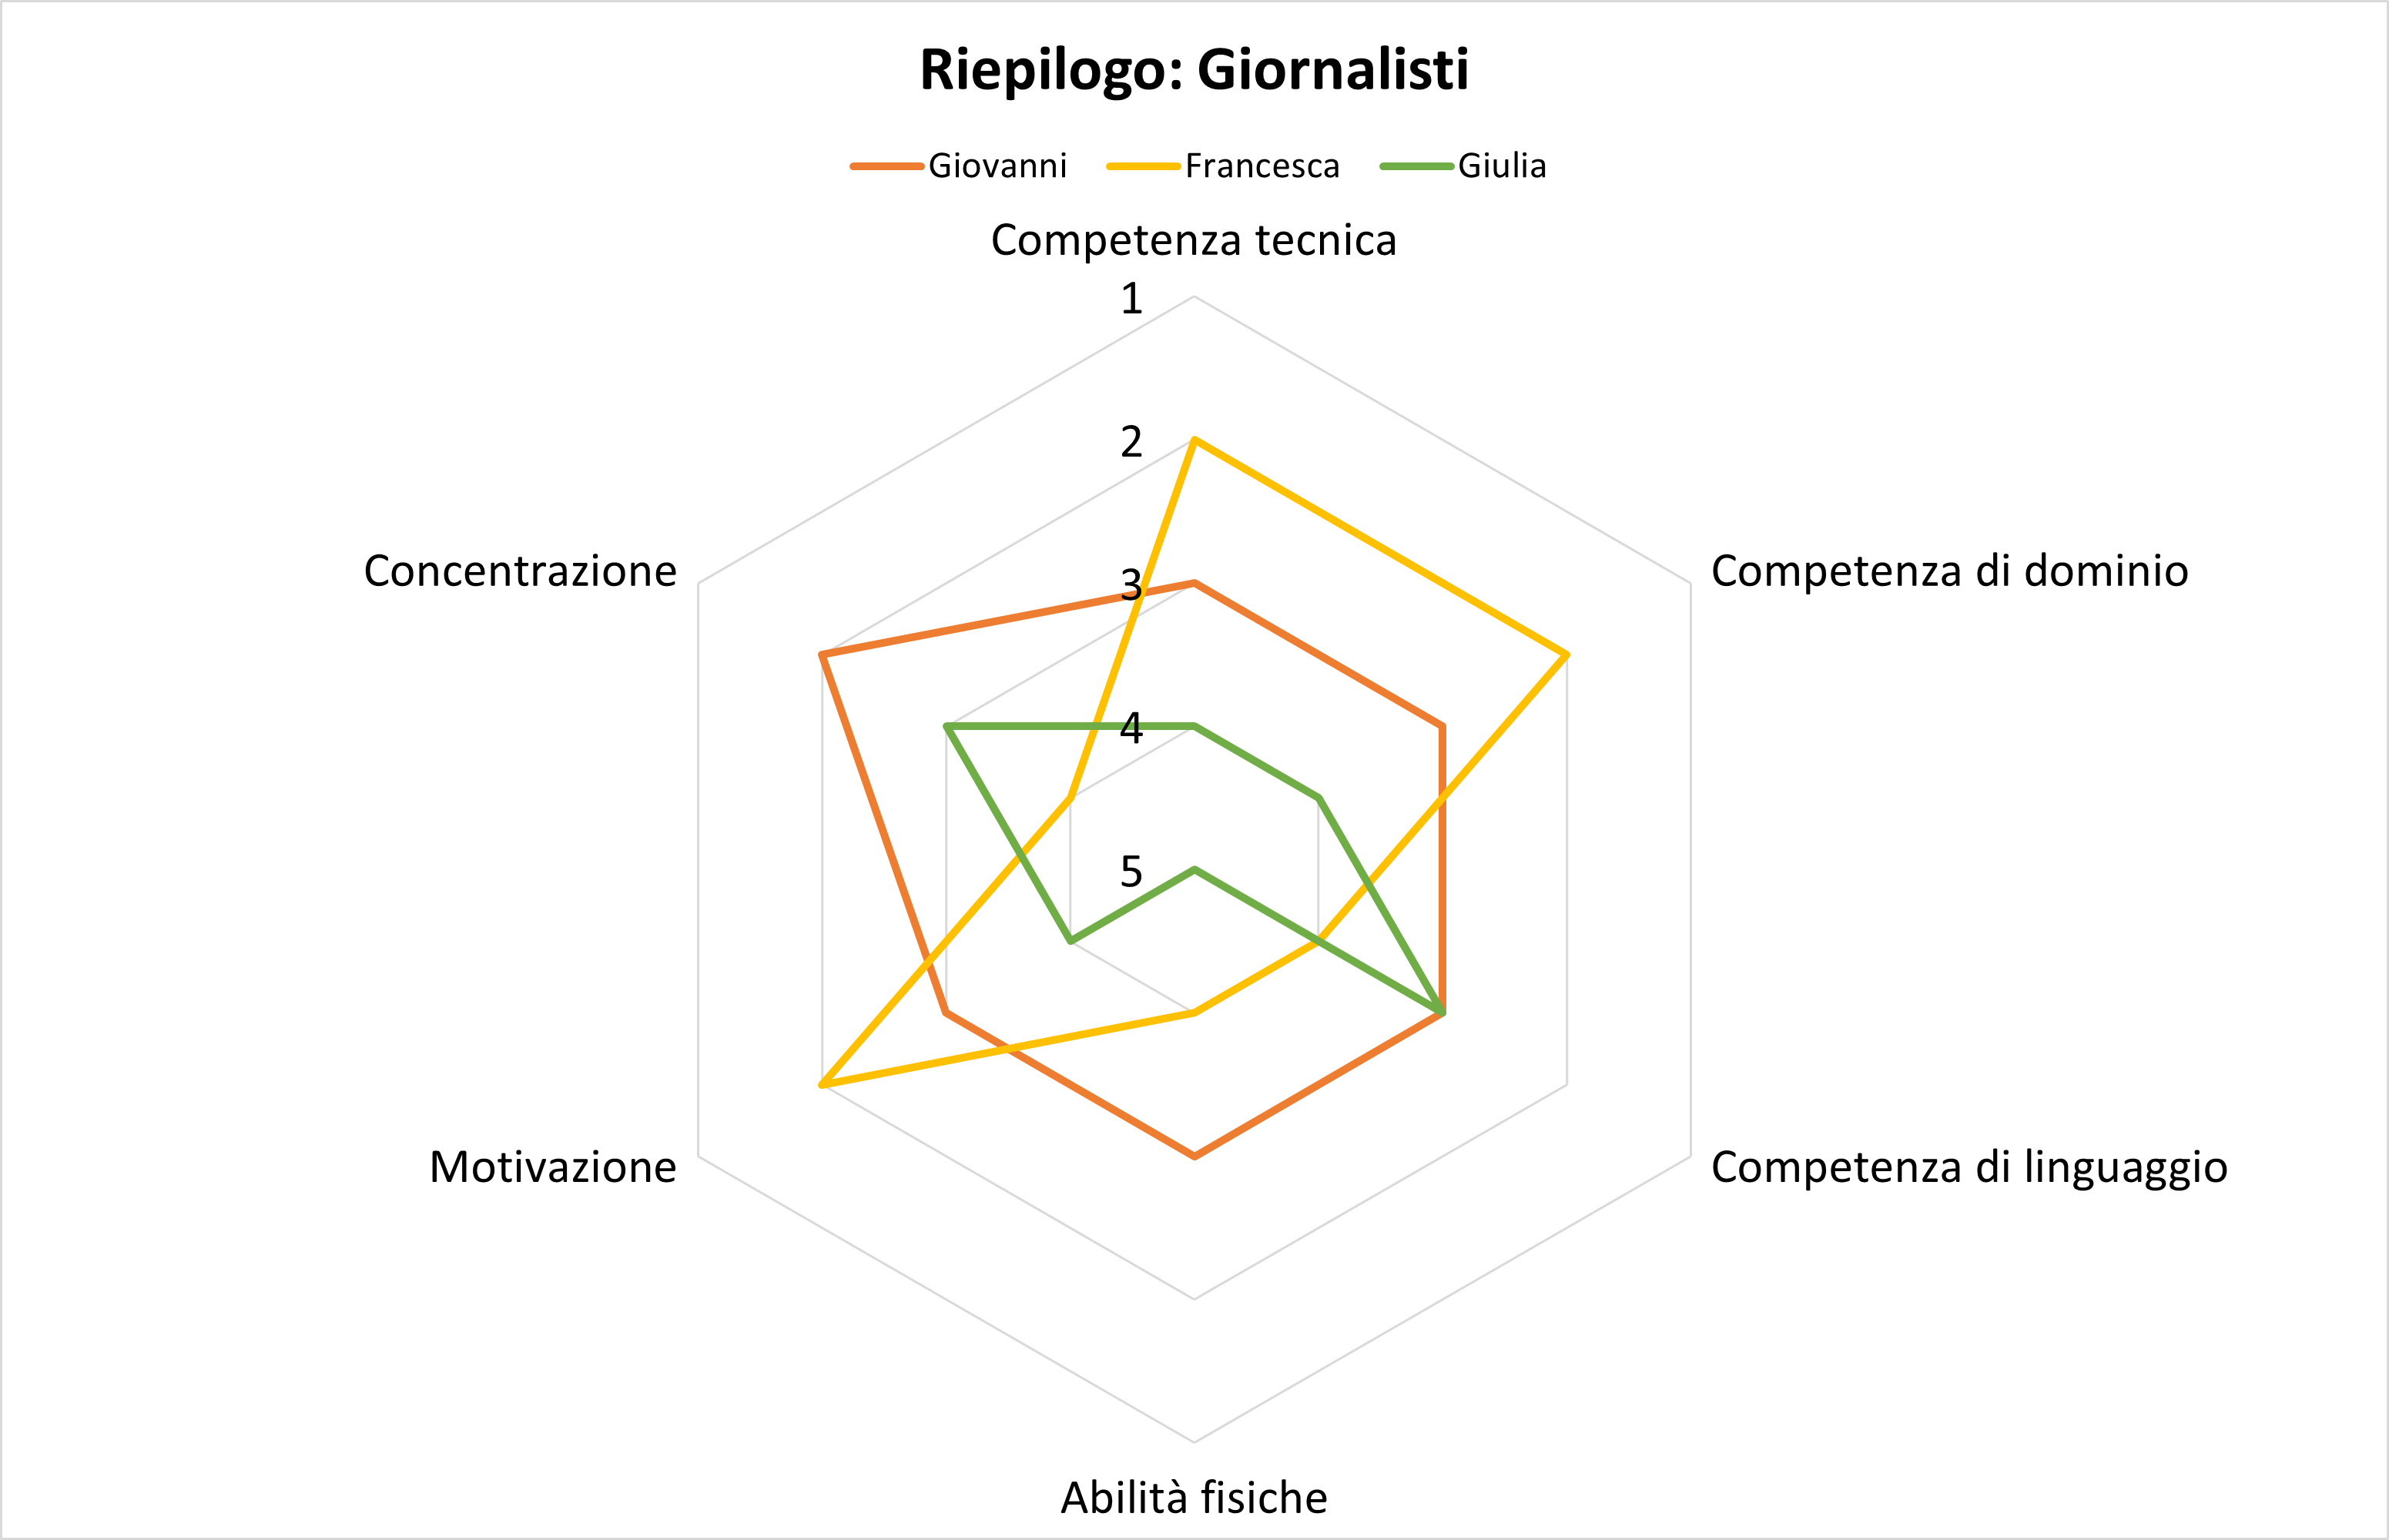
\includegraphics[width=0.5\columnwidth]{assets/images/proposta-design/caos/riepilogo-giornalisti}
    \caption{Diagramma C\&A di riepilogo sui giornalisti.}
\end{figure}

\noindent
Dal grafico relativo al cittadino esperto e al blogger, al contrario, è emersa una loro scarsa abilità fisica e competenza di linguaggio, il che ci ha portato a prevedere varie funzionalità in direzione dell'accessibilità, quali la possibilità di ingrandire i caratteri o espandere a schermo intero i grafici, e un registro familiare per le etichette e le spiegazioni.
\begin{figure}[H]
    \centering
    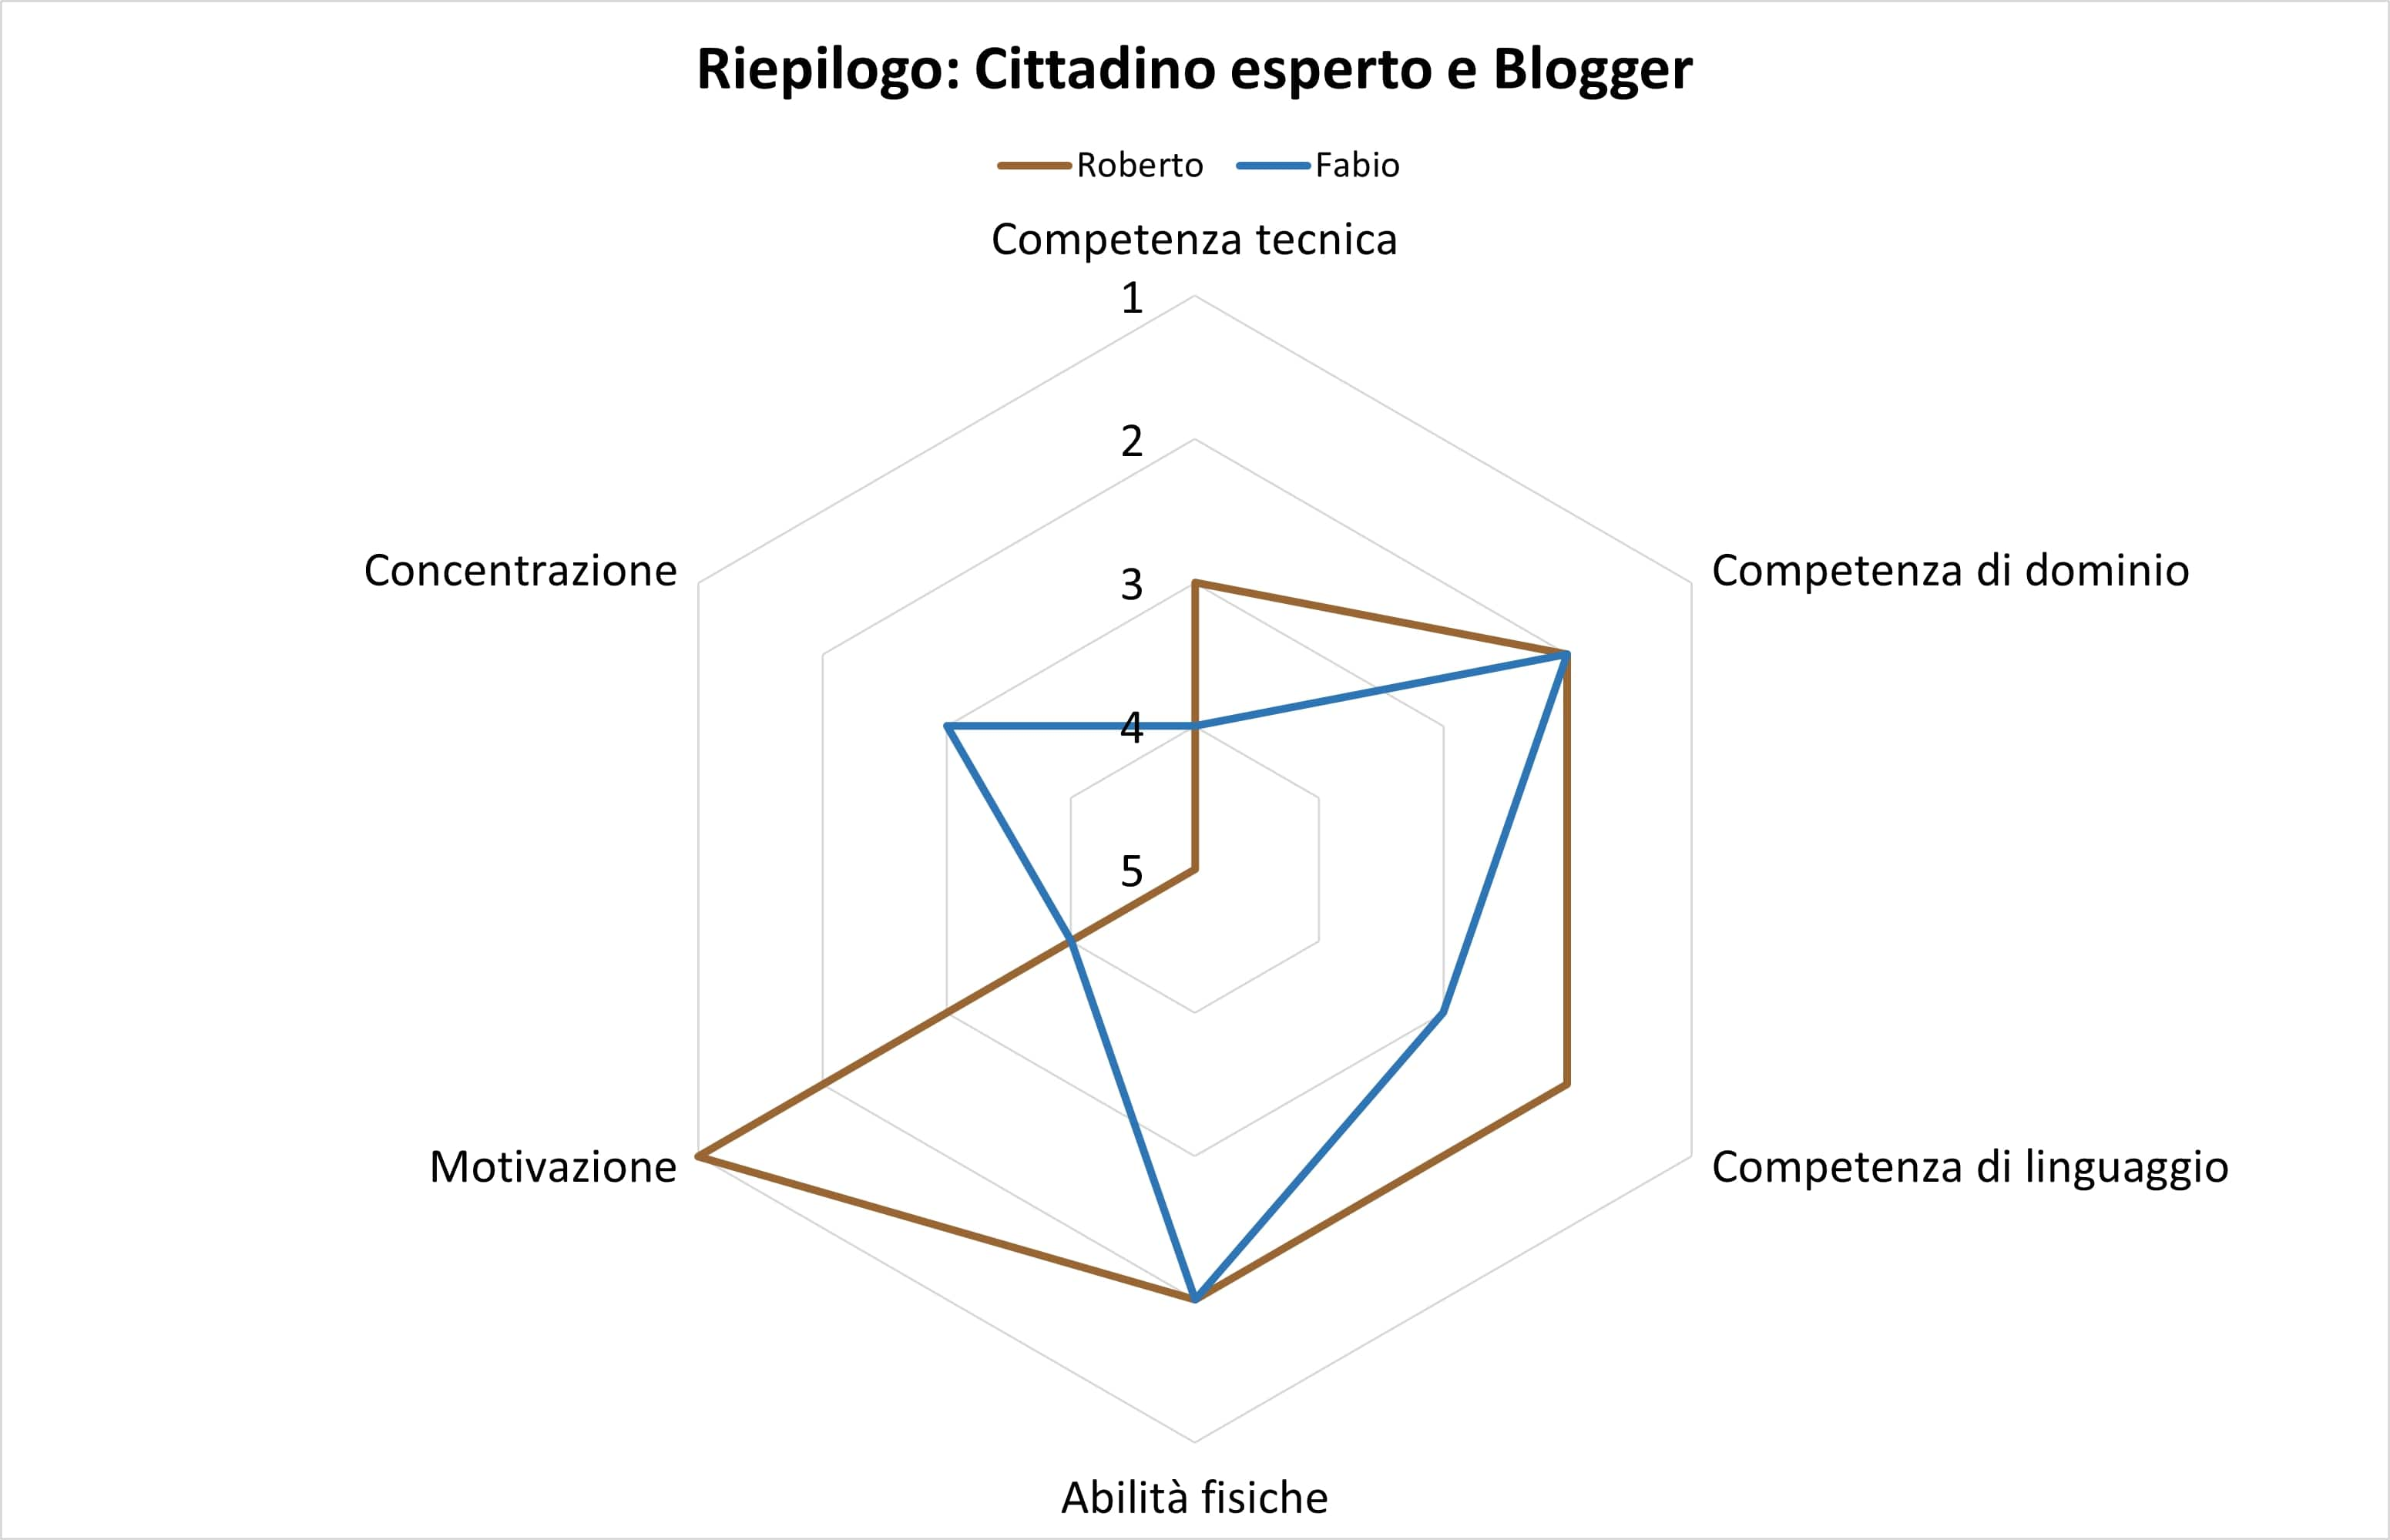
\includegraphics[width=0.5\columnwidth]{assets/images/proposta-design/caos/riepilogo-cittadini-altro}
    \caption{Diagramma C\&A di riepilogo sul blogger e il cittadino esperto.}
\end{figure}

\noindent
\paragraph{Scenari a partire dagli attori}\mbox{}\\
In seguito alla individuazione degli attori, il modello CAO=S ci ha richiesto di definire persona e scenari, per poi integrarli.
Abbiamo deciso di fare riferimento a quelli precedentemente elaborati durante lo Studio di fattibilità nel capitolo §3.
In particolare, per un'integrazione quanto più significativa, abbiamo rifinito alcuni aspetti marginali degli scenari, così da poter esaltare le peculiarità delle nostre persona mediante le attitudini e i comportamenti che hanno presentato nel realizzarli.\\
Gli scenari definiti in § sono:
\begin{itemize}
    \item Scenario 1: Analisi dei dati quotidiani sull'andamento dell'epidemia Covid-19 in Italia;
    \item Scenario 2: Analisi dei dati quotidiani sull'andamento dell'epidemia Covid-19 in Emilia Romagna;
    \item Scenario 3: Analisi sull'andamento del tasso di letalità e sulla distribuzione dei numeri dell'epidemia relativamente alle due settimane precedenti;
    \item Scenario 4: Confronto dell'andamento dell'epidemia nelle regioni Emilia Romagna, Veneto e Molise nelle precedenti due settimane;
    \item Scenario 5: Confronto dell'andamento dell'epidemia in Italia nel mese corrente rispetto ai due mesi precedenti.
\end{itemize}
Le persona caratterizzate in § sono:
\begin{itemize}
    \item Giornalista testata nazionale: Giovanni;
    \item Giornalista testata locale: Francesca;
    \item Giornalista di agenzia di stampa: Giulia;
    \item Blogger: Roberto;
    \item Cittadino esperto: Fabio;
    \item Utente che consulta dashboard da dispositivo mobile: Christian.
\end{itemize}
\noindent
\subparagraph{L'analisi quotidiana (scenario 1 svolto da Giulia)}\mbox{}\\
Giulia è una donna di 35 anni, laureata in Scienze Politiche all'Università di Milano.
Lavora per l'ANSA principalmente come ``fact-checker"; attualmente lavora da casa in quanto è ciò che l'agenzia ha imposto a causa della pandemia in atto.\\
Poco prima delle 17 accende il PC che le ha dato l'agenzia e si collega alla dashboard del DPC.
Alle 17 e 04 la dashboard le notifica che sono presenti dei dati aggiornati e quindi propone a Giulia di aggiornare la pagina.
Quando la pagina viene aggiornata vengono visualizzati i dati odierni; nella pagina che sta guardando vede e trascrive nel documento Word aperto in precedenza i dati di: numero di nuovi positivi, numero di deceduti, numero di nuovi ingressi in terapia intensiva e il rapporto tra nuovi positivi e tamponi effettuati.
Oltre a questi dati aggiunge all'articolo che sta scrivendo le immagini dei grafici che rappresentano l'andamento della pandemia.
Infine, per concludere la scrittura dell'articolo legge le note della dashboard dove c'è spiegato che la Liguria e la Valle d'Aosta hanno avuto problemi con la comunicazione dei dati e quindi aggiunge all'articolo anche quest'informazioni.
\noindent
\subparagraph{La situazione odierna della pandemia in Veneto (scenario 2 svolto da Francesca)}\mbox{}\\
Francesca è una donna di 36 anni di Mestre, laureatasi in Scienze della Comunicazione all'Università di Padova.\\
Lavora da sette anni presso la redazione del Gazzettino, in cui cerca di raccontare la propria regione e i suoi cittadini con passione, per fornire il proprio contributo diventato ancora più importante durante questa pandemia.\\
Sta per terminare la propria giornata di lavoro e si sta preparando per redigere l'articolo quotidiano sull'andamento della pandemia nella sua regione, il Veneto.\\
Vuole capire soprattutto se rispetto a ieri la situazione è migliorata, speranzosa, dopo una settimana in cui i contagi sono elevati. Si collega alla dashboard del DPC non appena nota che sono passate le 17.
Una volta aperta la dashboard, analizza i dati riportati per la regione: cerca il numero dei nuovi positivi, dei decessi, dei tamponi effettuati e quindi del tasso di positività. Può pertanto iniziare a redigere il suo articolo.\\
E' stata oggi una giornata ricca di video-conferenze, tra cui una con il Sindaco di Padova per intervistarlo su come l'Università e il comune stanno agevolando la frequentazione delle aule universitarie nonostante la possibilità di contagio, quindi non ha avuto modo di informarsi se fossero uscite ordinanze o dichiarazioni da parte del Presidente della Regione.
Approfitta della possibilità di vedere le ordinanze emanate nella sezione apposita della dashboard, scoprendone una nuova risalente alla mattina.
Dopo averla letta, esternamente alla dashboard, al ritorno visualizza una notifica che la informa che sono stati aggiornati alcuni dati, precedentemente comunicati errati.\\
Procede ad aggiornare il suo articolo, in cui poi intende raccontare anche di quanto ha parlato con il Sindaco.
\noindent
\subparagraph{L'articolo di approfondimento (scenario 3 svolto da Giovanni)}\mbox{}\\
Giovanni è un uomo di 53 anni di Fiumicino, felicemente sposato da 24 anni e con 2 figlie.\\
Dopo aver completato gli studi presso l'Università La Sapienza di Roma e aver fatto esperienza in giornali locali, lavora ormai da 19 anni presso il Corriere della Sera, dove ricopre il ruolo di redattore capo.
La sua posizione in redazione gli richiede la scrittura di articoli di approfondimento su temi di attualità: nel 2020, uno degli argomenti più accesi è la pandemia Covid-19, la quale, oltre a minacciare la sanità pubblica, sta stravolgendo gli assetti sociali, politici ed economici consolidatisi negli ultimi decenni.\\
Il 10 dicembre 2020 decide di redigere un articolo di analisi tramite cui fornire ai suoi lettori insight di valore circa il tasso di letalità e la distribuzione delle metriche epidemiologiche sui dati anagrafici, così da comunicare quali sono le categorie più a rischio.
Per acquisire le informazioni necessarie, si rivolge alla dashboard del DPC, divenuta negli ultimi mesi il suo punto principale di riferimento, tantoché ha creato anche una configurazione dell'interfaccia ritagliata sui bisogni informativi che di volta in volta ha per la stesura dei suoi articoli.
Anzitutto recupera, con uno sguardo immediato, il tasso di letalità, per poi richiedere i dati delle principali metriche, indicando che gli siano restituiti corredati dei dati anagrafici dei soggetti coinvolti, quali impiego, età e genere: dalla loro analisi, ravvisa una correlazione tra età e tasso di positività, secondo cui i soggetti più anziani sarebbero maggiormente esposti al contagio. 
\noindent
\subparagraph{Il confronto fra il Veneto e la vicina Emilia-Romagna (scenario 4 svolto da Roberto)}\mbox{}\\
La situazione della pandemia tra Veneto ed Emilia-Romagna sta avendo una uno sviluppo diametralmente opposto.
Roberto, un uomo di 30 anni che di mestiere fa il blogger e lo youtuber si è interessato a questo strano fatto dopo aver ricevuto un messaggio da un suo follower che gli chiede di approfondire il perché le due regioni avessero numeri così diversi.\\
Inizia le sue ricerche partendo dalla dashboard del DPC con la quale riesce a confrontare gli andamenti della pandemia per entrambe le regioni in maniera immediata, nota che effettivamente in Veneto la situazione è molto peggiore dell'Emilia Romagna in quanto sia il rapporto medio tra nuovi positivi e tamponi sia la media del numero di ospedalizzazioni giornaliere e anche i decessi cumulati sono  molto maggiori.
Roberto usa la dashboard anche per recuperarsi i vari provvedimenti presi dalle regioni e nota come in Veneto sono state introdotte più restrizioni solo nell'ultimo periodo. \\
Dopo essersi preso qualche appunto sui dati visualizzati e scaricate le immagini dei grafici scrive il testo per il video che pubblicherà il giorno seguente sul perché la situazione in Veneto sia molto peggio rispetto alla situazione in Emilia Romagna.
\noindent
\subparagraph{Comprensione profonda dei dati contro il sensazionalismo dei giornali (scenario 5 svolto da Fabio)}\mbox{}\\
L'estate del 2020, per gli italiani, è stata un momento di tregua e riscatto, covato ardentemente e a lungo nei difficili mesi all'inizio del 2020, imperversati dalla pandemia Covid-19: le calde giornate estive hanno registrato numeri molto contenuti per le varie metriche epidemiologiche (nuovi positivi, ingressi nelle terapie intensive, deceduti…); inoltre, le misure restrittive imposte dal Governo per contrastare la diffusione del contagio sono state minime e mirate.
Questa nuova situazione sociale ed epidemiologica ha persuaso importanti fette della popolazione a lasciarsi andare in comportamenti dall'alto rischio di contagio, come assembramenti e scarso, se non nullo utilizzo di strumenti di protezione individuale.
Ed ecco che sul finire di agosto, si sono iniziati a registrare cambi di direzione nelle tendenze decrescenti dei vari indicatori epidemiologici.\\
E' il 2 settembre 2020 e Fabio, docente di Informatica all'università G. D'Annunzio di Pescara, è appena rientrato da un viaggio in compagnia di Claudia, sua moglie da ben 25 anni, e dei suoi figli.
Fabio non appartiene alla fetta di popolazione noncurante di cui sopra: anzi, anche durante il viaggio appena trascorso, ha indossato la mascherina in ogni ambiente chiuso o affollato, invitando anche la sua famiglia a fare altrettanto; inoltre, si informa quotidianamente sull'andamento delle metriche.
Da qualche giorno, gli è capitato di imbattersi più volte nella lettura di articoli giornalistici sul tema che, invece di riportare il peggioramento in atto del quadro sanitario, presentano toni ottimistici e superficiali, rasentando inesattezze e sottostime della realtà.
In particolare, da più parti ha appurato che il numero di ospedalizzati sono diminuiti di un fattore di 10 rispetto a quelli registrati nel mese di maggio: questo dato gli sembra irrealistico, per cui si rivolge alla dashboard del DPC che solitamente consulta quando ha necessità di schiarirsi le idee.
Procede quindi col richiedere il dato dei nuovi casi positivi alla data corrente (2 settembre) e la dashboard gli restituisce 1.326, valore che replica quasi esattamente i 1.327 dell'8 maggio.
Focalizzandosi su queste due date confrontabili, richiede i dati dei ricoveri e trova 1.437 ricoverati con sintomi e 109 posti di terapia intensiva occupati del 2 settembre rispetto ai 14.636 e 1.168 del 9 maggio.
Guardando solo a questi valori assoluti, conclude che tra le due date esiste il rapporto di 1 a 10, millantato dai giornali.
Ancora non propriamente convinto, consulta siti istituzionali, alla ricerca di argomentazioni scientifiche circa l'analisi dei dati epidemiologici: scopre che le terapie intensive di un determinato giorno non sono espressione del numero dei nuovi casi del giorno stesso, ma del cumulato dei casi del mese precedente.
Ripete quindi la sua analisi sulla dashboard e trova i seguenti risultati: l'8 maggio i 14.636 ricoverati e le 1.168 terapie intensive riflettevano quindi gli 81.599 positivi rilevati a partire dall'8 aprile, mentre il 2 settembre i 1.437 ricoverati e le 109 terapie intensive erano ``figli" dei 23.286 casi rilevati a partire dal 3 agosto.
Alla luce di questa nuova consapevolezza, calcola che a maggio i ricoverati erano il 17,9\% dei casi dei 30 giorni precedenti e le terapie intensive l'1,4\%, mentre a settembre il dato è rispettivamente 6,1\% e 0,4\%.
Il rapporto cambia completamente rispetto a quello rilevato usando i valori assoluti del singolo giorno: è circa un terzo, non un decimo.
Fabio, acquisita questa nuova informazione, la comunica sui social network su cui è iscritto, corredando il suo post con un'immagine dei risultati comunicati direttamente dalla dashboard.
Ne parla quanto più in ogni occasione, in famiglia e con gli amici, al fine di aiutarli nel comprendere la reale situazione, certamente migliore di quella di maggio, ma non così rosea come si legge nei giornali, invitando sempre alla prevenzione del contagio.
\noindent
\subparagraph{L'informazione quotidiana (nessuno scenario riconducibile, svolto da Christian)}
Christian è un uomo di 34 anni che lavora come fattorino per un'agenzia di logistica.
Ha un appartamento a Torino vicino a una fermata della metropolitana e per raggiungere la propria sede di lavoro deve necessariamente prenderla quotidianamente.\\
A pranzo, quando è in pausa, è abituato ad informarsi sull'andamento della pandemia poiché sa che essa necessariamente influenza il suo lavoro.
Leggendo degli articoli presso uno dei giornali da cui solitamente si informa è venuto a conoscenza di questa fonte da cui i giornalisti attingono per i loro articoli.\\
Purtroppo però, accedendovi, scopre che non è fruibile per dispositivi mobili come il suo smartphone e quindi lo abbandona, tornando a leggere il suo articolo.
\noindent
\subparagraph{Caricamento quotidiano dei dati (nessuno scenario riconducibile, svolto dall'amministratore di database e dashboard)}
L'amministratore della base di dati collegata alla dashboard inserisce quotidianamente un'istanza per ciascuno dei seguenti concetti: andamento giornaliero nazionale, andamento del giorno di tutte e venti le regioni, andamento del giorno delle province, la situazione ad oggi nazionale, la situazione nelle venti regioni.\\
Per la creazione di questi dati non utilizza la dashboard ma un'altra interfaccia, quella del DBMS.